The results page displays a comprehensive overview of all the results from the
user's previous decompositions. This page allows the user to select up to five
decompositions for comparison purposes, providing the flexibility to mix and
match results from different runs of the tool.

\Cref{fig:results,fig:expanded_result} provide a visual representation of the
results page and showcase the user interface elements and features available on
this page, such as the list of decompositions, selection checkboxes, and any
other relevant information the underlying tool provides, like weigths, and
metadata.

\begin{figure*}[!htb]
  \centering
  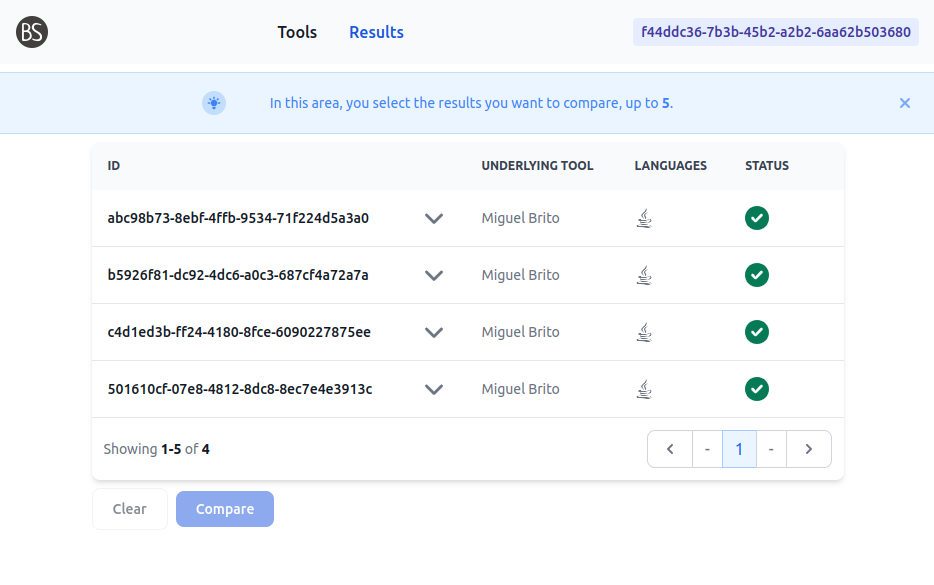
\includegraphics[width=\textwidth]{results}
  \caption{All Results}
  \label{fig:results}
\end{figure*}
\begin{figure*}[!htb]
  \centering
  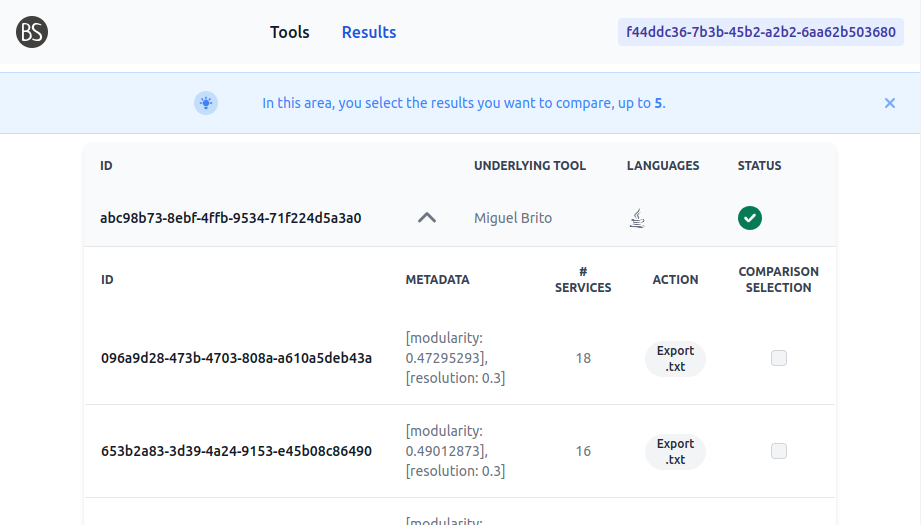
\includegraphics[width=\textwidth]{results_expanded}
  \caption{Expanded Result}
  \label{fig:expanded_result}
\end{figure*}
